% This file was created with tikzplotlib v0.10.1.
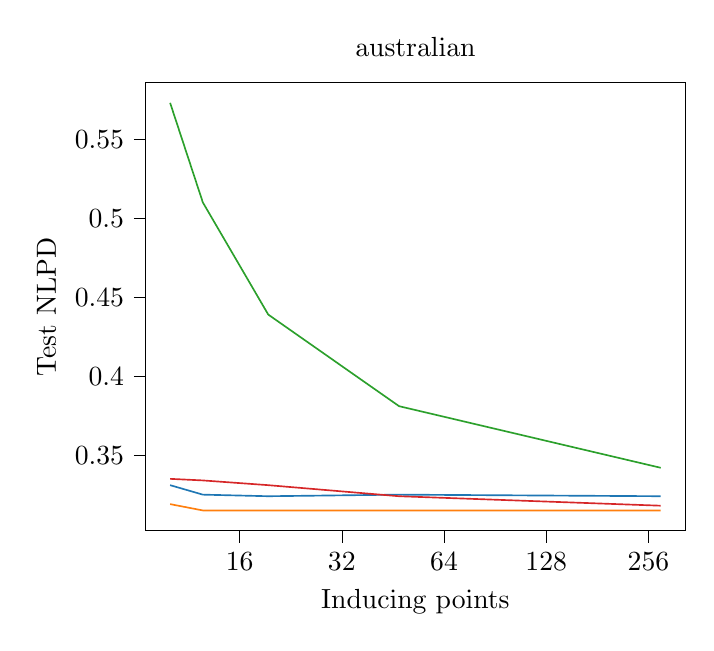
\begin{tikzpicture}

\definecolor{crimson2143940}{RGB}{214,39,40}
\definecolor{darkgray176}{RGB}{176,176,176}
\definecolor{darkorange25512714}{RGB}{255,127,14}
\definecolor{forestgreen4416044}{RGB}{44,160,44}
\definecolor{steelblue31119180}{RGB}{31,119,180}

\begin{axis}[
tick align=outside,
tick pos=left,
title={australian},
x grid style={darkgray176},
xlabel={Inducing points},
xmin=4, xmax=268,
xtick style={color=black},
xtick={0,50,100,150,200,250,300},
xticklabels={0,16,32,64,128,256,},
y grid style={darkgray176},
ylabel={Test NLPD},
ymin=0.3021, ymax=0.5859,
ytick style={color=black}
]
\addplot [semithick, steelblue31119180]
table {%
16 0.331
32 0.325
64 0.324
128 0.325
256 0.324
};
\addplot [semithick, darkorange25512714]
table {%
16 0.319
32 0.315
64 0.315
128 0.315
256 0.315
};
\addplot [semithick, forestgreen4416044]
table {%
16 0.573
32 0.51
64 0.439
128 0.381
256 0.342
};
\addplot [semithick, crimson2143940]
table {%
16 0.335
32 0.334
64 0.331
128 0.324
256 0.318
};
\end{axis}

\end{tikzpicture}
